\section{Results}\label{sec:results}

\subsection{RQ1: Pronunciation}
Table~\ref{tab:bench} and Fig.~\ref{fig:bench} give NepTTS-Bench results. Swar's pronunciation CER is 2.9\%; the next system is OmniVoice run with our studio prompt (4.3\%), then Indic-Speak Srijana (8.1\%) and ElevenLabs v3 (12.9\%). Among systems with published audio, Swar has the lowest pronunciation error in every benchmark category except newspaper ambiguities (4 sentences), where Indic-Speak Sagar is slightly lower (4.3 against 4.8). On standard CER Swar also leads, OmniVoice within 0.5 points. With the studio prompt, Swar does not lead on predicted naturalness: Indic-Speak Srijana scores UTMOS 3.97 and OmniVoice 3.93, against 3.82. With a read-style prompt in a podcast voice (Section~\ref{sec:voice}), Swar's demo voice Maya reaches UTMOS 4.09, the highest of any system, and beats Srijana on both error rates (7.45 and 4.52 against 10.25 and 8.12), but not OmniVoice (6.68 and 4.32). No single prompt leads on everything. The public NepaliMOS predictor puts every system between 2.88 and 3.05 (Swar 2.96, OmniVoice 2.98, Piper 3.05, Maya 2.88). The small paired differences are consistent across sentences, but the ranking does not follow intelligibility or the listener: Piper, with the most pronunciation errors, scores highest, and the voice our listener preferred scores lowest.

\begin{table}[t]\centering\small
\caption{NepTTS-Bench, 205 sentences: mean per-file CER (\%) and UTMOS. Our rows use today's frontend and one take; the Maya and Sabina rows use a read-style prompt chosen on development data. Other systems are their published or default-setting audio, scored identically.}\label{tab:bench}
\begin{tabular}{lrrr}\toprule
System & CER & Pron.\ CER & UTMOS\\\midrule
Swar, final model & \textbf{6.19} & \textbf{2.92} & 3.82\\
Swar, Maya voice & 7.45 & 4.52 & \textbf{4.09}\\
Swar, Sabina voice & 9.82 & 6.57 & 4.08\\
Swar, accent stage & 6.23 & 3.35 & 3.81\\
Swar, bilingual stage & 6.45 & 3.26 & 3.78\\
OmniVoice (our prompts) & 6.68 & 4.32 & 3.93\\
Indic-Speak Srijana & 10.25 & 8.12 & 3.97\\
Indic Parler-TTS Amrita & 11.70 & 9.51 & 3.26\\
Indic-Speak Sagar & 12.37 & 10.53 & 3.81\\
TingTing Subina & 13.39 & 11.25 & --\\
ElevenLabs v3 & 15.70 & 12.91 & --\\
Gemini & 15.31 & 15.03 & --\\
Piper & 18.68 & 17.00 & --\\\bottomrule
\end{tabular}
\end{table}

\begin{figure}[t]\centering
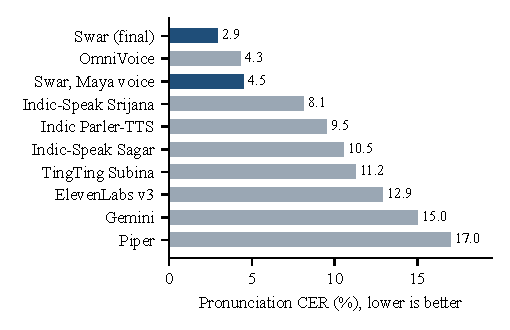
\includegraphics[width=\columnwidth]{fig_bench.pdf}
\caption{Pronunciation CER on NepTTS-Bench (lower is better).}\label{fig:bench}
\end{figure}

On the studio test, Swar's mean per-file CER is 8.95 against 10.93 for the human recordings of the same sentences (names: 22.1 against 21.9), with UTMOS 3.72 against 3.62. Against the real take of the same sentence, the clone's ECAPA similarity is 0.78, its F0 correlation 0.49, and its pace within 13\%.

\subsection{RQ2: Cloning from Phone Audio}
On 50 unseen IndicVoices-R speakers, ECAPA accepts 97\% of clones as the target speaker, against 98\% of genuine second recordings (equal error rate 2\%), and WavLM-SV~\citep{wavlm} accepts 91\% of both. On FLEURS, the final model reaches similarity 0.694 and CER 4.6, against 0.681 and 5.3 for OmniVoice, whose predicted naturalness is higher (UTMOS 2.49 against 2.39). FLEURS prompts are noisy (the real recordings score UTMOS 2.24) and the model copies the noise. Denoising the prompt with DeepFilterNet3~\citep{deepfilternet}, with the removal capped at 18\,dB (chosen on FLEURS validation speakers), gives CER 4.55, similarity 0.691 and UTMOS 2.67: first on all three. Full denoising sounds cleaner still (UTMOS $+0.3$ on validation) but costs similarity and CER.

On WhatsApp voice notes, the clone of a held-out sentence matches the person's real clip at 0.767, against 0.771 between that person's own clips, for a speaker with five minutes of notes; for a speaker whose notes were recorded months apart, the figures are 0.598 and 0.630. From a single 30-second window, similarity is 0.74, 0.70 or 0.62 depending on the window: slow, careful speech gave the lowest. Enrolment from a 30.6 s upload takes 23.5 s on one L4 GPU, and a best-of-4 sentence about 10 s.

\subsection{RQ3: The Frontend}
\paragraph{Pronunciation layers.} With the accent-stage model, adding the mined fixes, the Nepal pronunciation layer and the English layer lowered NepTTS-Bench pronunciation CER from 3.98 to 3.13 at unchanged standard CER (6.14 to 6.15), as expected for a layer whose effect is on sounds the standard metric does not separate. On the 30 code-switched sentences, English in Latin letters gives CER 43.9; the English layer brings it to 6.4 (OmniVoice: 12.1), and the reviewed spellings to 5.6 with the final model.

\paragraph{Held final vowels.} Fig.~\ref{fig:vowel} shows the duration of the held sound for five words. The halanta form lengthens \np{खान} from 108 to 155 ms and \np{जान} from 92 to 112 ms. With the take check, 22 of 24 rendered demo lines have a held sound of at least 120 ms.

\begin{figure}[t]\centering
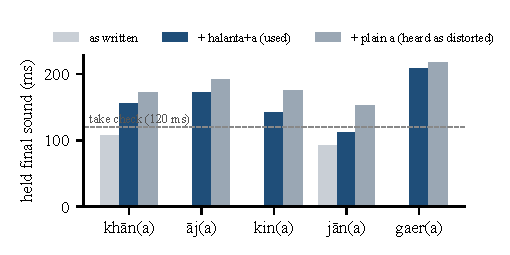
\includegraphics[width=\columnwidth]{fig_vowel.pdf}
\caption{Duration of the held word-final sound, forced alignment, 8 takes per spelling. Missing bars: not measured as written. The plain form was heard as distorted.}\label{fig:vowel}
\end{figure}

\paragraph{English.} Fig.~\ref{fig:english} compares four ways of producing full English sentences. English text with a Nepali prompt is unusable (best-take WER 59.5\%). English text with a prompt of the same speaker speaking English, found in the podcasts, is intelligible (5.8\%) and scores the highest UTMOS, but the native listener found it hard to understand. Nepali-letter English with the original spellings is intelligible to Whisper (0.3\%) yet was heard as broken, for example \emph{everyone} as ``eveeonee''. With the reviewed spellings every voice reaches 0.0\% on the best take, the line that failed for every voice before (\emph{bought a beautiful new jacket}) included, and the listener accepted it. Two English fine-tunes, LibriTTS-R speech paired with Nepali-letter text and the speakers' own 344 English clips, changed nothing measurable.

\begin{figure}[t]\centering
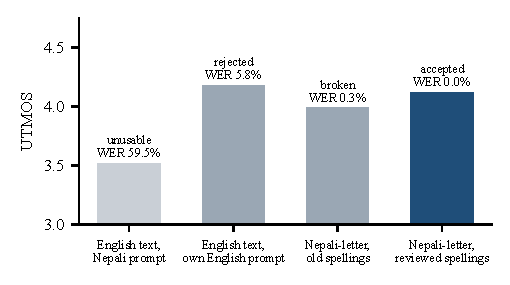
\includegraphics[width=\columnwidth]{fig_english.pdf}
\caption{Full English sentences: UTMOS, best-take Whisper WER and the native listener's verdict for four routes. The routes used different voices and numbers of takes (see text), so the figure compares routes, not voices.}\label{fig:english}
\end{figure}

\subsection{RQ4: Training vs Prompting}
Eight preset voices, four female and four male, come from one studio speaker and the permitted podcasts. Table~\ref{tab:pod} compares the base model with the model fine-tuned on the speakers' own podcast speech, on pieces held out from training. Similarity rises by 0.005 on average, pronunciation CER moves in both directions, and UTMOS is level; cloning of unseen speakers is unchanged (similarity 0.650 to 0.652, CER 6.4 to 6.3). Full fine-tunes on the two studio speakers gave the same picture (F0 correlation 0.42--0.47 against 0.49 for the base). The base model already clones these voices from a prompt; we keep the fine-tuned model because it is never worse.

\begin{table}[t]\centering\small
\caption{Clone against the speaker's real held-out piece, base / fine-tuned, 8 pieces per voice, one take (5 of 10 voices).}\label{tab:pod}
\begin{tabular}{lccc}\toprule
Voice & Similarity & Pron.\ CER & UTMOS\\\midrule
Podcast host (m) & .626 / .636 & 1.9 / 2.2 & 3.11 / 3.11\\
Guest 1 (m) & .753 / .760 & 3.6 / 2.1 & 3.54 / 3.52\\
Podcast host A (f) & .697 / .698 & 2.7 / 3.3 & 3.95 / 3.88\\
Interview A (f) & .725 / .729 & 3.3 / 3.2 & 3.76 / 3.89\\
Interview B (f) & .671 / .678 & 3.3 / 2.9 & 3.93 / 3.85\\\bottomrule
\end{tabular}
\end{table}

\subsection{Prompt Voice and Naturalness}\label{sec:voice}
Predicted naturalness depends mostly on the prompt. On 60 held-out Rasa sentences, the studio prompt gives UTMOS 3.55 and the podcast voices 3.89--3.95, at higher CER (6.9--7.2 against 4.6) because the podcast prompts are fast casual talk. A read-style prompt, made by letting the model read training-split sentences in the podcast voice and keeping the take that clones best on other training sentences, keeps the voice and lowers CER to 5.4--5.9 at UTMOS 4.07--4.16. Short phrases are the exception: F5 copies the prompt's pace, and on 40 short phrases (four seeds each) every podcast voice makes 40--80\% more errors than the studio voice (14.3--18.5 against 10.3) for $+0.2$ UTMOS; slowing the voice does not remove the gap. NepTTS-Bench is 94\% phrases under 30 letters, which is why the Maya and Sabina rows in Table~\ref{tab:bench} trade pronunciation for naturalness. Our own recogniser, Kriti, does not see this gap on the same audio (pronunciation CER 4.6 for the studio voice, 4.1--4.4 for the podcast voices), and neither did the native listener: in a blind choice over 12 short phrases, the studio voice was never preferred, Maya won 8 and Nisha 4; among male voices Aarav and Sujan won 5 each and the studio voice none. The short-phrase penalty is therefore at least partly MMS's, though the benchmark is scored with it. Maya and Aarav are the demo voices. Best-of-4 takes by our own recogniser, more flow steps, output enhancement (resemble-enhance~\citep{resembleenhance} raises UTMOS on long sentences by 0.24 but not on short phrases), loudness normalisation and silence padding did not change this.

\subsection{Human Evaluation}
A pilot with one native rater (17 sentences per system, 1--5 scale, loudness-matched) gave the human recordings 3.75, Swar 3.12, OmniVoice 3.06, Piper 3.06, TingTing 2.82 and ElevenLabs 2.76. A blind public listening test with naturalness and pronunciation ratings, A/B comparisons and a vote over the eight preset voices is built; its results will be added in a revision.
